\documentclass{article}
\usepackage{graphicx}
\usepackage{hyperref}

\begin{document}

\title{PREP-BRAMS Instalation  and User's Manual}
\author{Luiz Flávio Rodrigues}

\maketitle

\begin{abstract}
This document contains instruction to install and use the preprocessor for BRAM'S Model.
\end{abstract}

\section{Instalation}
Follow the instructions in following sections to proced PRE-BRAM's instalation. For all instalation we recomend You to create an install's directory in Your home area.

\begin{verbatim}
cd ~
mkdir install
\end{verbatim}

\subsection{Grib2}

Go to folder You created, download and unpack the grib2 API from NCEP:

\begin{verbatim}
cd ~/install
wget https://www.ftp.cpc.ncep.noaa.gov/wd51we/wgrib2/wgrib2.tgz
tar -zxvf wgrib2.tgz
cd grib2
\end{verbatim}

Using your preferred editor, edit the makefile, search and modify as shown below:

\begin{verbatim}
USE_NETCDF3=0     
USE_NETCDF4=0     
USE_REGEX=1     
USE_TIGGE=1     
USE_MYSQL=0     
USE_IPOLATES=3     
USE_SPECTRAL=0     
USE_UDF=0     
USE_OPENMP=0     
USE_PROJ4=0     
USE_WMO_VALIDATION=0     
DISABLE_TIMEZONE=0     
MAKE_FTN_API=1     
DISABLE_ALARM=0     
USE_G2CLIB=0     
USE_PNG=0     
USE_JASPER=0     
USE_AEC=0
\end{verbatim}

Make the files (in this case the compilers are gfortran/gcc, You can try others):

\begin{verbatim}
make CC=gcc FC=gfortran
make CC=gcc FC=gfortran lib
cd ..
sudo mv grib2 /opt
\end{verbatim}

\textbf{Note: In this case the files are moved to /opt folder. If You have no sudo permission You can choose other one in Your home area.}

Check if libraries and modules was compiled:

\begin{verbatim}
ls /opt/grib2/lib
\end{verbatim}

You must see the following libraries and files: 
\begin{verbatim}
libgeo.a libip2_d.a libwgrib2.a libwgrib2_api.a libwgrib2x.a wgrib2api.mod wgrib2lowapi.mod
\end{verbatim}

\subsection{Zlib}

Goto install folder and get the file

\begin{verbatim}
cd ~/install
wget https://www.zlib.net/zlib-1.2.11.tar.xz
\end{verbatim}

Unpack the file and go to folder

\begin{verbatim}
xz -d zlib-1.2.11.tar.xz
tar -xvf zlib-1.2.11.tar
cd zlib-1.2.11
\end{verbatim}

Compile and install

\begin{verbatim}
CC=gcc ./configure --prefix=/opt/zlib
make
sudo make install
\end{verbatim}

\textbf{Note: In this case the files are moved to /opt folder. If You have no sudo permission You can choose other one in Your home area.}

\subsection{hdf5}

In your browser go to \href{https://www.hdfgroup.org/downloads/hdf5/source-code/}{https://www.hdfgroup.org/downloads/hdf5/source-code/} and download the newest source code to install folder (or Download Folder) You create previously. (In example the version is hdf5-1.10.6.tar.bz2). In most cases the file is downloaded to ~/Download folder.

Go to folder, Unpack and compile HDF5

\begin{verbatim}
cd ~/install
mv ~/Downloads/hdf5-1.10.6.tar.bz2 .
bunzip2 hdf5-1.10.6.tar.bz2
tar -xvf hdf5-1.10.6.tar
cd hdf5-1.10.6.tar.bz2
./configure --prefix=/opt/hdf5 CC=gcc FC=gfortran --with-zlib=/opt/zlib --enable-parallel --enable-fortran
make
sudo make install
\end{verbatim}

\textbf{Notes:}
\begin{enumerate}
	\item \textbf{In this case the files are moved to /opt folder. If You have no sudo permission You can choose other one in Your home area.}
	\item \textbf{If You will use hdf5 for parallel environments we suggest You use mpif90/mpicc instead gfortran and gcc - Pay attention because You must have installed mpich3 or other environment before compiling hdf5}
	\item \textbf{Case You want to use hdf5 with parallel mpi refer to BRAMS manual to know how to install it!}
\end{enumerate}

\subsection{NetCDF C (Base Library)}

In your browser go to \href{https://www.unidata.ucar.edu/downloads/netcdf/}{https://www.unidata.ucar.edu/downloads/netcdf/} and download the newest source code 
   to install folder (or Download Folder) You create previously. (In example the version is netcdf-c-4.7.3.tar.gz)
   
Go to folder, unpack and compile

\begin{verbatim}
cd ~/install
mv ~/Downloads/netcdf-c-4.7.3.tar.gz .
tar -xzvf netcdf-c-4.7.3.tar.gz
cd netcdf-c-4.7.3
./configure --prefix=/opt/netcdfc FC=gfortran CC=gcc LT_SYS_LIBRARY_PATH=/opt/hdf5/lib CFLAGS='-I/opt/hdf5/include' LIBS='-L/opt/hdf5/lib'
make
sudo make install
\end{verbatim}

\textbf{Notes:}
\begin{enumerate}
	\item \textbf{In this case the files are moved to /opt folder. If You have no sudo permission You can choose other one in Your home area.}
	\item \textbf{If You will use netCDF C for parallel environments we suggest You use mpif90/mpicc instead gfortran and gcc - Pay attention because You must have installed mpich3 or other environment before compiling it}
	\item \textbf{Point the LIBRARY, Include and LIBS to HDF5 path installed previously }
\end{enumerate}
   
\subsection{NetCDF Fortran}

In your browser go to \href{https://www.unidata.ucar.edu/downloads/netcdf/}{https://www.unidata.ucar.edu/downloads/netcdf/} and download the newest source code to install folder (or Download Folder) You create previously. (In example the version is netcdf-fortran-4.5.2.tar.gz)
   
Go to folder, unpack and compile

\begin{verbatim}
cd ~/install
mv ~/Downloads/netcdf-fortran-4.5.2.tar.gz .
tar -xzvf netcdf-fortran-4.5.2.tar.gz
cd netcdf-fortran-4.5.2
export LD_LIBRARY_PATH=/opt/netcdfc/lib:/opt/hdf5/lib:$LD_LIBRARY_PATH
export CC=/opt/mpich3/bin/mpicc
export FC=/opt/mpich3/bin/mpif90
export CPPFLAGS="-I/opt/netcdfc/include -I/opt/hdf5/include"
export LDFLAGS="-L/opt/netcdfc/lib -L/opt/hdf5/lib"
./configure --prefix=/opt/netcdff
make
sudo make install
\end{verbatim}

\textbf{Notes:}
\begin{enumerate}
	\item \textbf{In this case the files are moved to /opt folder. If You have no sudo permission You can choose other one in Your home area.}
	\item \textbf{If You will use netCDF Fortran for parallel environments we suggest You use mpif90/mpicc instead gfortran and gcc - Pay attention because You must have installed mpich3 or other environment before compiling it}
	\item \textbf{Point the LIBRARY PATH, CPPFLAGS, LDFLAGS,Include and LIBS to HDF5 path installed previously }
\end{enumerate}

\subsection{Pre Brams}

Go to PRE-BRAMS build directory 

\begin{verbatim}
cd ~/BRAMS-5.5/auxProgs/PRE-BRAMS/build
\end{verbatim}

Edit the file paths.mk and change the lines accordingly

\begin{verbatim}
CHEM_MECH=RELACS_TUV
GRIB2_PATH=/opt/grib2/
NETCDFC_PATH=/opt/netcdfc
NETCDFF_PATH=/opt/netcdff
\end{verbatim}

There are just one include.mk.\textbf{XXX} file, for gnu compiler (gcc/gfortran). where \textbf{XXX} is the compiler environment (GNU, etc). If You will use another one please, copy it for a new and edit the lines. 

\begin{verbatim}
FC           =gfortran
FC_OPTS      = -DUSEPARALELL=$(USEPARALELL) -DUSEGRIB=$(USEGRIB) -ffree-form -ffree-line-length-none
FLOADER      =gfortran
\end{verbatim}

Change to compiler You want and save it. If compiler is ifort, include.mk.intel e.g.:

\begin{verbatim}
FC           =ifort
FC_OPTS      = -DUSEPARALELL=$(USEPARALELL) -DUSEGRIB=$(USEGRIB)
FLOADER      =ifort
\end{verbatim}

\textbf{Notes:}
\begin{enumerate}
	\item \textbf{All defined path must be compliance with previously installed libraries.}
	\item \textbf{All the libraries must use the same compiler You choose.}
	\item \textbf{The make available by default is for include.mk.gnu - gfortran/gcc}
\end{enumerate}

Compile the PRE

\begin{verbatim}
make OPT=gnu
\end{verbatim}

\textbf{Notes:}
\begin{enumerate}
	\item \textbf{use gnu only for include.mk.gnu}
\end{enumerate}

\section{How it works}

The PRE BRAMS get information from GFS/NCEP model's data and from CAMS's Model's 10 years chem climatology, transform, regrid and concatenate them on a single group of files that will be initial and borders conditions to the BRAM's Model. The output files are write in bin grads (Cola) format with grads descriptors file.

The GFS data is in grib2 format, and the CAMS Climatology data are in NetCDF4 format.

PRE BRAMS read a namelist file named 'pre.nml' thats informs the dates, files and directories to be processed. The chemical and aerosol species equivalence between BRAMS chem1\_list inside model are translated into some species from CAMS by using the table of equivalence (file 'equivalence'). 

The operator only need to edit the namelist pre.nml to run the PRE. The CAMS Climatology and Table of equivalence are fixed and tunned for an specific set of chemistry mechanism.

The PRE do not run in parallel mode, use it only ina  single processor. 


\begin{figure}
    \centering
    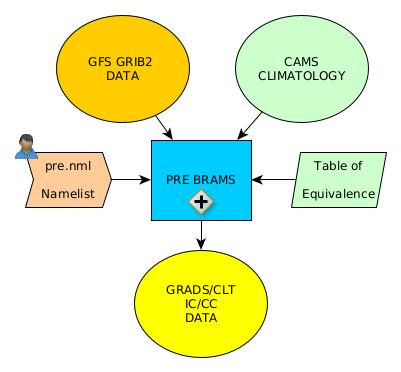
\includegraphics[width=3.0in]{graf1.jpg}
    \caption{PRE BRAMS Scheme}
    \label{simulationfigure}
\end{figure}

\section{Getting the data}

For run the PRE you need 2 sets of files, CAMS climatology files and GRIB2 GFS files. create a data folder (in example we use data) to put all datafiles and goto it

\begin{verbatim}
mkdir ~/data
cd ~/data
\end{verbatim}

\subsection{CAMS Climatology}

Get the cams climatology on: \href{http://ftp.cptec.inpe.br/pesquisa/bramsrd/DATA\_CAMS/}{http://ftp.cptec.inpe.br/pesquisa/bramsrd/DATA\_CAMS/}. The files have the format: \textbf{MMM}-CAMS-EC-2010-2019-AMS.nc where \textbf{MMM} are the month (JAN,FEB,...,DEC).

\begin{verbatim}
wget http://ftp.cptec.inpe.br/pesquisa/bramsrd/DATA_CAMS/JAN-CAMS-EC-2010-2019-AMS.nc
wget http://ftp.cptec.inpe.br/pesquisa/bramsrd/DATA_CAMS/FEB-CAMS-EC-2010-2019-AMS.nc
wget http://ftp.cptec.inpe.br/pesquisa/bramsrd/DATA_CAMS/MAR-CAMS-EC-2010-2019-AMS.nc
wget http://ftp.cptec.inpe.br/pesquisa/bramsrd/DATA_CAMS/APR-CAMS-EC-2010-2019-AMS.nc
wget http://ftp.cptec.inpe.br/pesquisa/bramsrd/DATA_CAMS/MAY-CAMS-EC-2010-2019-AMS.nc
wget http://ftp.cptec.inpe.br/pesquisa/bramsrd/DATA_CAMS/JUN-CAMS-EC-2010-2019-AMS.nc
wget http://ftp.cptec.inpe.br/pesquisa/bramsrd/DATA_CAMS/JUL-CAMS-EC-2010-2019-AMS.nc
wget http://ftp.cptec.inpe.br/pesquisa/bramsrd/DATA_CAMS/AUG-CAMS-EC-2010-2019-AMS.nc
wget http://ftp.cptec.inpe.br/pesquisa/bramsrd/DATA_CAMS/SEP-CAMS-EC-2010-2019-AMS.nc
wget http://ftp.cptec.inpe.br/pesquisa/bramsrd/DATA_CAMS/OCT-CAMS-EC-2010-2019-AMS.nc
wget http://ftp.cptec.inpe.br/pesquisa/bramsrd/DATA_CAMS/NOV-CAMS-EC-2010-2019-AMS.nc
wget http://ftp.cptec.inpe.br/pesquisa/bramsrd/DATA_CAMS/DEC-CAMS-EC-2010-2019-AMS.nc
\end{verbatim}

\textbf{Notes:}
\begin{enumerate}
	\item \textbf{The data must be downloaded just once}
\end{enumerate}

\subsection{GFS data}

Get the GFS data from nomads on https://nomads.ncep.noaa.gov/pub/data/nccf/com/gfs/prod/gfs.\textbf{YYYYMMDD/HH}/gfs.t00z.pgrb2.0p25.f\textbf{TTT} where: \linebreak
\textbf{YYYY} - Year with 4 digits \linebreak \textbf{MM} - Month with 2 digits \linebreak \textbf{DD} - Day with 2 digits \linebreak \textbf{HH} - Hour (00,06,12 or 18) of run \linebreak \textbf{TTT} - Time for analysis (from 000 until 384).\linebreak

get the data You have interest. E.g. If You want to generate data for 24h, 6/6 hours  begining 01Sep2020

\begin{verbatim}
wget https://nomads.ncep.noaa.gov/pub/data/nccf/com/gfs/prod/gfs.20200901/00/gfs.t00z.pgrb2.0p25.f000 -O gfs.t00z.pgrb2.0p25.f000.2020090100.grib2
wget https://nomads.ncep.noaa.gov/pub/data/nccf/com/gfs/prod/gfs.20200901/00/gfs.t00z.pgrb2.0p25.f006 -O gfs.t00z.pgrb2.0p25.f002.2020090100.grib2
wget https://nomads.ncep.noaa.gov/pub/data/nccf/com/gfs/prod/gfs.20200901/00/gfs.t00z.pgrb2.0p25.f012 -O gfs.t00z.pgrb2.0p25.f012.2020090100.grib2
wget https://nomads.ncep.noaa.gov/pub/data/nccf/com/gfs/prod/gfs.20200901/00/gfs.t00z.pgrb2.0p25.f018 -O gfs.t00z.pgrb2.0p25.f018.2020090100.grib2
wget https://nomads.ncep.noaa.gov/pub/data/nccf/com/gfs/prod/gfs.20200901/00/gfs.t00z.pgrb2.0p25.f024 -O gfs.t00z.pgrb2.0p25.f024.2020090100.grib2
\end{verbatim}

\textbf{Notes:}
\begin{enumerate}
	\item \textbf{The name of file from NOMADS dont have the date of analysis. Put a suffix in filename to inform the analisys date. Above we are using ".2020090100.grib2"}
	\item \textbf{You can choose other data folder You want}
	\item \textbf{You must Download Cams Climatology just once. Save it for use in future.}
	\item \textbf{You must download all cams climatology for every months You need. Check the initial and final dates of your simulation.}
\end{enumerate}

\section{namelist for PRE}

You need edit the namelist for each period You want.

Go to bin folder

\begin{verbatim}
cd ~/BRAMS-5.5/auxProgs/PRE-BRAMS/bin
\end{verbatim}

Using Your editor, edit Namelist file 'pre.nml' to your run:

\begin{verbatim}
init_year  = 2020,
init_month = 09,
init_day   = 01,
init_hour  = 0,
final_year = 2020,
final_month= 09,
final_day =  02,
final_hour = 0,
...
step  = 6, !Timestep in hours
...
atmos_prefix ='gfs.t00z.pgrb2.0p25.f',
atmos_sufix  ='.2020090100.grib2',
atmos_idir   ='~/dados/',
...
chem_idir  = '~/dados/',
chem1_prefix ='',
chem1_sufix  ='-CAMS-EC-2010-2019-AMS',
...
out_prefix = 'IC',
out_sufix  = '',
out_dir    = '~/bin/datain/GRADS/',
\end{verbatim}

\textbf{Notes:}
\begin{enumerate}
	\item \textbf{The example above is for the date of 01Sep2020 with 24h simulation}
	\item \textbf{The output directory is set to put the initial conditions in your BRAMS run folder:~/bin/datain/GRADS/ }
\end{enumerate}

\section{Run PRE}

just run the executable:

\begin{verbatim}
./PREP_1.0
\end{verbatim}


\end{document}